%\documentclass{article}
%\usepackage{amsmath
    %              ,siunitx
    %           ,fancyhdr
    %               ,amssymb
    %               ,centernot
    %               %,tikz
    %              %,tikzsymbols
    %               %,pgfplots
    %              ,graphicx
    %               ,csquotes
    %               ,bm
    %               ,tocloft
    %               ,titlesec
    %               ,parskip
    %               ,leftidx
    %               ,hyperref}
%\usepackage[margin=1in]{geometry}
%\usepackage[version=4]{mhchem}

%\cftsetindents{section}{0.75em}{6em}
%\renewcommand{\cftsecpresnum}{Lecture }  % Sets up the table of contents and section heading
%\renewcommand{\cftdot}{.}
%\renewcommand{\cftsecleader}{\cftdotfill{\cftdotsep}}
%\titlelabel{Lecture \thetitle}
%\setcounter{section}{0}

%\pgfplotsset{width=5cm,compat=1.9}  % sets version and standard width for pgfplots, I just copied values from the internet
%\graphicspath{ {./Images/} }  % Tells graphicx where images are stored relative to this document
%\hypersetup{hidelinks}  % makes links invisible in table of contents

%\newcommand{\vh}[1]{\vec{\hat{#1}}}
%\renewcommand{\vec}[1]{\underline{#1}}
%\renewcommand{\vec}[1]{\bm{#1}}
%\newcommand{\vv}[1]{\vec{#1}}
%\newcommand{\ve}[1]{\vec{\hat{e}_{#1}}}
%\newcommand{\pd}[3][]{\frac{\partial^{#1}{#2}}{\partial{#3}^{#1}}}
%\newcommand{\dv}[3][]{\frac{d^{#1}{#2}}{d{#3}^{#1}}}
%\newcommand{\pdiff}[2][]{\frac{\partial^{#1}}{\partial{#2}^{#1}}}
%\newcommand{\diff}[2][]{\frac{d^{#1}}{d{#2}^{#1}}}
%\newcommand{\A}{\forall\,}
%\newcommand{\E}{\exists\,}
%\newcommand{\bb}[1]{\mathbb{#1}}
%\newcommand{\cc}[1]{\overline{#1}}
%\newcommand{\hb}{\hbar}

%%%%%%%%%%%%%%%%%%%%%%%%%%%%%%%%%%%%%%%%%
% Copy these commands to the complete document:
%\newcommand{\aparticle}{\ensuremath{\alpha} particle}
%\newcommand{\aparticles}{\ensuremath{\alpha} particles}
%\newcommand{\bparticle}{\ensuremath{\beta} particle}
%\newcommand{\bparticles}{\ensuremath{\beta} particles}
%\newcommand{\bpparticle}{\ensuremath{\beta^+} particle}
%\newcommand{\bmparticle}{\ensuremath{\beta^-} particle}
%\newcommand{\proton}{\ensuremath{\mathrm{p}}}
%\newcommand{\neutron}{\ensuremath{\mathrm{n}}}
%\newcommand{\electron}{\ensuremath{\mathrm{e}^-}}
%\newcommand{\positron}{\ensuremath{\mathrm{e}^+}}
%\newcommand{\neutrino}[1][]{\ensuremath{\nu_{#1}}}
%\newcommand{\antineutrino}[1][]{\ensuremath{\bar\nu_{#1}}}
%\newcommand{\muonm}{\ensuremath{\mu^-}}
%\newcommand{\muonp}{\ensuremath{\mu^+}}
%\newcommand{\tauonm}{\ensuremath{\tau^-}}
%\newcommand{\tauonp}{\ensuremath{\tau^+}}
%\newcommand{\piplus}{\ensuremath{\pi^+}}
%\newcommand{\piminus}{\ensuremath{\pi^-}}
%\newcommand{\pizero}{\ensuremath{\pi^0}}
%\newcommand{\kplus}{\ensuremath{\mathrm{k^+}}}
%\newcommand{\kminus}{\ensuremath{\mathrm{k^-}}}
%\newcommand{\kzero}{\ensuremath{\mathrm{k^0}}}
%\newcommand{\antikzero}{\ensuremath{\mathrm{\bar k^0}}}
%\newcommand{\up}{\ensuremath{\mathrm{u}}}
%\newcommand{\down}{\ensuremath{\mathrm{d}}}
%\newcommand{\charm}{\ensuremath{\mathrm{c}}}
%\newcommand{\strange}{\ensuremath{\mathrm{s}}}
%\newcommand{\topquark}{\ensuremath{\mathrm{t}}}
%\newcommand{\bottom}{\ensuremath{\mathrm{b}}}
%\newcommand{\quark}{\ensuremath{\mathrm{q}}}
%\newcommand{\antiquark}{\ensuremath{\mathrm{\bar q}}}
%\newcommand{\red}{\ensuremath{\mathrm{r}}}
%\newcommand{\green}{\ensuremath{\mathrm{g}}}
%\newcommand{\blue}{\ensuremath{\mathrm{b}}}
%\newcommand{\wplus}{\ensuremath{\mathrm{W^+}}}
%\newcommand{\wminus}{\ensuremath{\mathrm{W^-}}}
%\newcommand{\wpm}{\ensuremath{\mathrm{W^\pm}}}
%\newcommand{\zboson}{\ensuremath{\mathrm{Z^0}}}

%\DeclareSIUnit{\solarmass}{\ensuremath{\mathrm{M_\odot}}}
%%%%%%%%%%%%%%%%%%%%%%%%%%%%%%%%%%%%%%%%
%
%
%\newcounter{example}[section]
%\newenvironment{example}[1][]{\refstepcounter{example}\vspace{-0.2cm}
%\subsubsection*{Example~\thesection.\theexample} \rmfamily}{\par}
%
%%The stuff below sets up header/footer and shrinks margins
%\pagestyle{fancy}
%\lhead{Willoughby Seago}
%\rhead{Physics 1B lecture notes}
%\cfoot{Page \thepage}
%\renewcommand{\headrulewidth}{0.4pt}
%\renewcommand{\footrulewidth}{0.4pt}
%\setlength{\parindent}{0pt}

%The stuff below is used to set up the title
%\title{Physics 1B Lecture Notes}
%\author{Willoughby Seago}
%\date{18 January 2019}
%
%\begin{document}
\part{Nuclear, Particle and Astro Physics}
\section{}

\SI{1}{eV} is the energy gained when one electron is accelerated through a potential difference of \SI{1}{V}.\linebreak \SI{1}{eV}=\num{1.6e-19}\,\si{J}. Using energy-mass equivalency it is possible to write mass as \(m=E/c^2\). This means that \si{MeV/c^{2}} is a unit of mass. Another unit of mass is the atomic mass unit \si{u}, which is defined as \(1/12\) the mass of \ce{^12_6C}.

\begin{center}
\begin{tabular}{cccc}\hline
 & Mass in \si{kg} & Mass in \si{eV/c^2} & Mass in \si{u} \\\hline
Proton & \num{1.673e-27}\,\si{kg} & \SI{938.3}{MeV/c^2} & \SI{1.007}{u}\\
Neutron & \num{1.675e-27}\,\si{kg} & \SI{939.6}{MeV/c^2} & \SI{1.009}{u}\\
Electron & \num{9.11e-31}\,\si{kg} & \SI{511}{KeV/c^2} & \SI{0.0005}{u}\\
\SI{1}{kg} & \SI{1}{kg} & \num{5.61e35}\,\si{eV/c^2} & \num{6.022e26}\,\si{u}\\
\SI{1}{MeV/c^2} & \num{1.78e-30}\,\si{kg} & \SI{1}{MeV/c^2} & \SI{0.0011}{u}\\
\SI{1}{u} & \num{1.66e-27}{kg} & \SI{931.49}{MeV/c^2} & \SI{1}{u}\\\hline
\end{tabular}
\end{center}

In 1897 electrons were discovered and JJ Thompson developed the plum pudding model. In 1908 Geiger and Marsden (supervised by Rutherford) discovered that the mass was concentrated at the center of the atom.

\begin{example}
An \(\alpha\) particle has mass \(\approx\SI{4000}{MeV/c^2}\) and kinetic energy \(\approx\SI{5}{MeV}\). What is the \(\alpha\) particle's velocity?

\(E\ll m/c^2\) so it is non-relativistic.
\[E=\frac12mv^2\implies\SI{5}{MeV}=\frac12(\SI{4000}{MeV/c^2})v^2\]
\[\frac{\SI{10}{MeV}}{\SI{4000}{MeV}}=\frac{v^2}{\si{c^2}}\]
\[\frac{v^2}{\si{c^2}}=\frac{1}{400}\]
\[v=\frac{\si{c}}{20}=\SI{15000}{km s^{-1}}\]
A good check to do now is that \(v\ll c\) so it is definitely non-relativistic.
\end{example}
\begin{example}
What energy electron do you need to probe a proton?

A photon has a diameter of approximately \SI{1}{fm}, so we need electrons with wavelength of the same size.

\[p=\frac{h}{\lambda},\qquad\lambda\approx\SI{1}{fm}\]
\[p=\num{6.63e-19}\,\si{Js/m}=\SI{4.14}{eVs/m}\]
\[c=\num{3e8}\,\si{m/s}\implies\si{s/m}=\num{3e8}\,\si{/c}\]
\[p=\num{1.23e9}\,\si{eV/c}=\SI{1.23}{GeV/c}\]
\[E^2=p^2\mathrm{c}^2+m_0^2c^4\]
\[p=\SI{1.23}{GeV/c}\implies p^2c^2=(\SI{1.23}{GeV})^2\]
\[m_0=\SI{511}{keV/c^2}\implies m_0^2c^4=(\SI{511}{keV})^2\]
\[E^2=(\SI{1.23}{GeV})^2+(\SI{511}{keV})^2=\SI{1.23}{GeV^2}\]
So when \(E\gg m\) we get \(E=pc\) just as it does for a photon. Hence the energy required to probe a proton is \(\SI{1.11}{GeV}\).
\end{example}

\section{}

Nuclei are described by two numbers, the atomic number \(Z\), which is the number of protons, and the atomic mass \(A\) which is the number of nucleons. The number of neutrons is \(N=A-Z\). The radius of an average atom is \(10^{-10}\,\si{m}\). The radius of a nucleon is \(\approx\SI{1}{fm}=10^{-15}\,\si{m}\). Nuclear volume is proportional to the radius cubed, which is proportional to the number of nucleons. This results in a nuclear radius given by \(\num{1.2e-15}A^{1/3}\,\si{m}\).

The mass of an atom is less than the sum of the mass of its constituent parts. This mass difference results in the binding energy of the nucleus. If the mass of the nucleus is \(M(A,Z)\), then the binding energy \(BE\) is given by
\[BE=[Zm_p+(A-Z)m_n-M(A,Z)]c^2\]
The graph below shows the nuclear binding energy per nucleon

\begin{center}
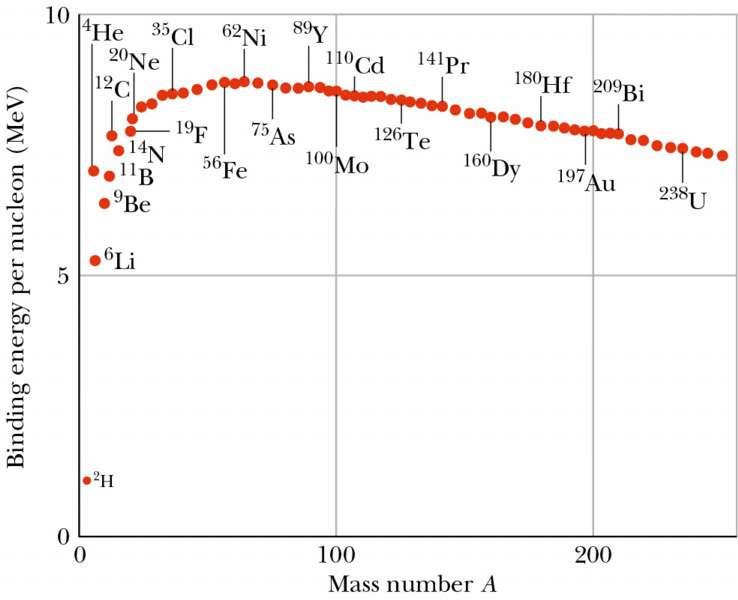
\includegraphics{BindingEnergyPerNucleon}
\end{center}

The graph peaks at \ce{^56Fe}. This is the most stable isotope. Isotopes to the left of \ce{^56Fe} relase energy by fusion. Isotopes to the right of \ce{^56Fe} release energy by fission.

The force that binds the nucleons is the strong force. The graph below shows the nucleon-nucleon potential \(U(r)\) and the magnitude of the force is given by \(F=-\dv Ur\). It can be seen that the strong force is repulsive under about \SI{1}{fm} and attractive from \SI{1}{fm} to about \SI{3}{fm} and beyond \SI{3}{fm} has little or no effect.

\begin{center}
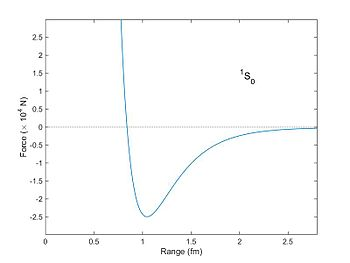
\includegraphics[scale=0.5]{StrongForce}
\end{center}

The most widely accepted model for how forces are mediated is that virtual particles are exchanged, this means that particles are created and travel between other particles carrying momentum and charge. This is allowed as long as \(\Delta E\Delta t\ge\hb/2\).

\begin{example}
A force is mediated by the exchange of virtual pions of mass \SI{140}{MeV/c^2}. How long can these particles exist for (ignoring relativistic effects)?

\begin{align*}
\Delta E\Delta t&>\hb\\
\Delta t&>\frac{\hb}{\SI{140}{MeV/c^2}}\\
\Delta t&>\frac{\num{1.05e-34}\,\si{Js}}{\num{140e6}\cdot\num{1.6e-19}\,\si{J}}\\
\Delta t&>\num{4.7e-34}\,\si{s}
\end{align*}
\end{example}

\section{}

\subsection*{Alpha Decay}

An \aparticle is a \ce{_2^4He} nucleus. \(\alpha\) decay happens when a large, unstable nucleus breaks into a smaller, more stable nucleus and an \aparticle, as in the example below:
\[\leftidx{_Z^A}{X}{}\ce{->}\leftidx{_{Z-4}^{A-2}}{X'}{}+\alpha\]
\subsubsection*{Conserved Quantities}
\begin{itemize}
\item Number of protons
\item Number of neutrons
\item Charge
\item Energy
\begin{itemize}
\item Mass before is larger than the mass after
\item Excess mass is turned into kinetic energy
\item Both the \aparticle and daughter nucleus have the same magnitude of momentum
\item The kinetic energy and velocity of the \aparticle are greater than the daughter nucleus'
\end{itemize}
\end{itemize}

Within \SI{1}{fm} of the nucleus the \aparticle is bound to the nucleus, outside of this distance the potential is very high and then decreases exponentialy. For \(\alpha\) decay the \aparticle must quantum tunnel through this energy barrier. Outside of the range of the strong force the potential is given by
\[U=\frac{1}{4\pi\varepsilon_0}\frac{Z_1Z_2}{r}\]
 Inside the barrier the \aparticle has ``negative energy''. This just means that there is something weird with complex numbers going on here.
 
The \aparticle has a charge of +2 so it interacts a lot with matter. This means that \aparticles are stopped by skin or paper.

\(\alpha\) decay is due to the strong force.

\subsection*{Beta Decay}

A \bmparticle is an electron and a \bmparticle is a positron. The decay occuring with \(\beta^-\) decay is
\[\leftidx{^Z_A}{\mathrm{X}}{}\ce{->}\leftidx{_{\hphantom{{}+1}A}^{Z+1}}{\mathrm{X}'}{}+\electron+\antineutrino[e]\]
\[\neutron\ce{->}\proton+\electron+\antineutrino[e]\]

\(\beta^+\) decay:
\[\leftidx{^Z_A}{\mathrm{X}}{}\ce{->}\leftidx{_{\hphantom{{}-1}A}^{Z-1}}{\mathrm{X}'}{}+\positron+\neutrino[e]\]
\[\proton\ce{->}\neutron+\positron+\neutrino[e]\]

Electron capture:
\[\leftidx{^Z_A}{\mathrm{X}}{}+\electron\ce{->}\leftidx{^{Z-1}_{\hphantom{{}-1}A}}{\mathrm{X}'}{}+\neutrino[e]\]
\[\proton+\electron\ce{->}\neutron+\neutrino[e]\]

\bparticles are less massive and have a lower magnitude of charge than \aparticles. This means that they interact with matter less. Consequently they need a few milimeters of aluminium to stop them.

\subsection*{Gamma Decay}

\begin{center}
\begin{tabular}{c|ccc}
Part of the spectrum & Visible & x-rays & gamma rays\\\hline
Typical energy measured in & \si{eV}& \si{keV} & \si{MeV}
\end{tabular}
\end{center}

Like electrons, nuclei also have excited states but since the radius is much less than for an atom the energy of these excited states is much greater. This means that decays of nuclei to ground states tend to have energies in the \si{MeV}s so they are in the gamma ray part of the spectrum. To stop a gamma ray a few inches of lead are needed.

\section{}

\subsection*{Spontaneous Fission}

Spontaneous fission occurs when a heavy, unstable nucleus splits into two smaller, individualy more stable nuclei. Typicaly the two daughter nuclei aren't the same mass. Often neutrons are produced at the same time. This is a slow process.

\subsection*{Induced Fission}

A neutron is fired at \ce{^235U} which makes \ce{^236U} which has a very short half life and quickly decays into two daughter nuclei and some neutrons. The number of neutrons produced depends on the daughter nuclei produced. If on average more than one neutron is produced then a chain reaction will occur. Typically \SI{200}{MeV} of energy is released per fission event. This corresponds to about \SI{0.2}{u} of mass being converted to energy. A \SI{1}{GW} power station requires about \SI{1}{g} of mass to be converted to energy per day which means approximately \SI{1.2}{kg} of \ce{^235} is used per day.

\subsection*{Fusion}

The most common fusion reaction on earth is deuterium (\ce{D}/\ce{^2H}) and tritium (\ce{T}/\ce{^3H}). This results in the reaction below
\[\mathrm{T+D}\ce{->^4He}+\neutron\]
This reaction releases \SI{17.6}{MeV} of energy. This is known as D--T fusion.  What actually occurs is that \ce{^5He} is produced but because its half life is less than \(10^{-15}\,\si{s}\) it immediately falls apart into \ce{^4He} and a neutron. The mass of the LHS of the reaction is about \SI{5.03}{u} and the mass of the RHS is about \SI{5.01}{u}. This means \SI{0.02}{u} of mass is converted to energy.

Fusion also occurs in the sun. The most common process at this stage in the suns life is
\begin{align*}
\ce{^1H}+\ce{^1H}&\ce{->}\ce{^2H} & (\text{Slow})\\
\ce{^1H}+\ce{^2H}&\ce{->}\ce{^3He} & (\text{Fast})\\
\ce{^3He}+\ce{^3He}&\ce{->}\ce{^4He}+2\ce{^1H} & (\text{Fast})
\end{align*}
The first step is the rate determining step. This reaction takes about 1 billion years. The sun is the equivalent of 100 billion nuclear bombs per second. Every second the sun converts \SI{655}{Mton} of hydrogen to \SI{650}{Mton} of helium.

In bigger stars another common cycle is the CNO cycle where several isotopes of carbon, nitrogen and oxygen are produced along with other smaller particles. It cycles around and ends up with energy being released but the same elements being present.

\subsection*{Particle Physics}

\begin{center}
\begin{tabular}{ccc}\hline
Particle & Size (\si{m}) & Relative size\\\hline
Atom & \(10^{-10}\) & 1\\[0.2em]
Nuclei & \(10^{-14}\) & \(\frac{1}{10000}\)\\[0.2em]
Nucleon & \(10^{-15}\) & \(\frac{1}{100000}\)\\[0.2em]
Quarks/leptons & \(<10^{-18}\) & \(<\frac{1}{100000000}\)\\\hline
\end{tabular}
\end{center}

We believe quarks and leptons are ``point like'' and have no substructure. We can't get individual quarks by themselves due to quark confinement. We have to defer that quarks exist from their influence on measurements such as scattering, decays and bound systems.

To measure small scales we need very large energies. From c. 1910 we have used cosmic rays and radioactive decays for this, from c. 1940 we have also used particle accelerators. Originally cloud chambers were used to detect these particles. Now more sensitive equipment such as ATLAS and CMS is used.

\section{}

Dirac proposed a new equation which took into account quantum mechanics and special relativity. This gave the energy of a particle as
\[E^2=p^2c^2+m^2c^4\]
\[E=\pm\sqrt{p^2c^2+m^2c^4}\]
If \(E>0\) then this is an ordinary particle. The negative energy gave rise to the possibility of antiparticles which were later shown to exist. This shows that every particle has a corresponding antiparticle. To the best of our knowledge antiparticles act just like particles traveling backwards in time.

Positrons (antielectrons) were discovered when a path in a cloud chamber in a magnetic field had equal radius of curvature (therefore momentum and mass) but opposite direction of curvature to the paths known to be caused by electrons. This could only happen if the positron had opposite charge to the electron since the curvature in a magnetic field is described by
\[\vv F=q(\vv E+\vv v\times\vv B)\]

The muon was discovered as it had a much larger radius of curvature (so less curvature) than an electron but was in the same direction (so a muon is negative). The mass of a muon is approximately 200 times the mass of an electron. Muons don't react strongly with protons but do react by the EM force and weak force. It was originally thought to be an exchange particle for the strong force but is too heavy.

The pion was discovered after the muon and is the exchange particle for the strong force. It has a mass of about \SI{140}{MeV/c^2}. It interacts by the strong force. Pions can have a charge of -1, 0 or +1. Pions decay to muons
\[\piminus\ce{->}\muonm+\antineutrino[\mu]\]
\[\piplus\ce{->}\muonp+\neutrino[\mu]\]
\(\pizero\)s are slightly more massive than \(\piminus\) or \(\piplus\).

Particles are characterised by
\begin{itemize}
\item Charge (\(\pm 1\) or 0)
\item How they interact
\begin{itemize}
\item Strong force
\item EM
\item Weak force
\end{itemize}
\item How they decay
\item Mass
\end{itemize}

\section{}

\subsection*{Deep Inelastic Scattering}

Deep inelastic scattering is a process similar to Rutherford scattering. High energies are used and photons or electrons instead of \aparticles. The beam of particles is concentrated on a singular proton or neutron. Most of the beam goes straight through the proton but occasionally there is scattering. The results suggest a substructure split into 3 parts. It isn't possible to knock single quarks out but occasionally jets of particles are produced. The interactions are all due to EM which we understand well.

\subsection*{Resonance}

Nuclei are closed and bound systems with energy levels typically measured in \si{MeV}. Each nucleus has a series of excited states. Some states correspond to the motion of individual neuclons where as other correspond to the motion of all neucleons. The details are very complicated as it is a strongly interacting many body problem. The only solutions that we have are numerical.

\ce{^1H} has no resonances, \ce{^4He} has its first non-ground state at \SI{20}{MeV} above the ground state.

Individual neucleons also can have excited states since they are a closed, bound system of three quarks. The energies of these states are typically measured in \si{Gev}. In particle physics these excited states are sometimes known as new particles rather than resonances of existing particles.

Most quark systems have 2 (mesons, quark--antiquark system) or 3 (hadrons) quarks. 4,5 and 6 quark systems do exist but aren't on this course. The quark systems with more than 3 quarks have very short half lifes.

There are 6 flavours of quark made of 3 generations. They also all have antiparticles. They are up quarks \up, down quarks \down, charm quarks \charm, strange quarks \strange, top quarks \topquark and bottom quarks \bottom. Some of the particles these can make are shown in the table below.

\begin{center}
\begin{tabular}{cc|cc}\hline
Particle & Quark Structure & Particle & Quark Structure\\\hline
Proton & uud & Antiproton & \(\mathrm{\bar u\bar u\bar d}\)\\
Neutron & ddu & Antineutron & \(\mathrm{\bar d\bar d\bar u}\)\\
\piplus & \(\mathrm{u\bar d}\) & \piminus & \(\mathrm{\bar ud}\)\\
\pizero & \(\mathrm{u\bar u/d\bar d}\) & Average \pizero & \(\frac{\mathrm{u\bar u-d\bar d}}{\sqrt2}\)\\
\kzero & \(\mathrm{d\bar s}\) & \(\mathrm{J/\psi}\) & \(\mathrm{c\bar c}\)\\\hline
\end{tabular}
\end{center}

If the charge of a particle \(x\) is denoted \(q_x\) then we can calculate \(q_\up\) and \(q_\down\) from \(q_\proton\) and \(q_\neutron\)
\begin{align*}
q_\up + q_\up + q_\down&=1\\
q_\up + q_\down + q_\down &=0\\
\end{align*}
\[\implies q_\up =+\frac 23,\quad q_\down=-\frac 13\]
Similar calculations give \(q_\up=q_\charm=q_\topquark=+\frac 23\) and \(q_\down=q_\strange=q_\bottom=-\frac 13\)

Up and down quarks link to electrons, antielectrons, electron neutrinos and antielectron neutrinos.

Charm and strange quarks link to muons, antimuons, muon neutrinos and antimuon neutrinos.

Top and bottom quarks link to tauons, antitauons, tauon neutrinos and antitauon neutrinos.

\begin{center}
\begin{tabular}{c|cccccc}\hline
Class & Generation 1 & Mass & Generation 2 & Mass & Generation 3 & Mass\\\hline
Lepton & e & \SI{0.5}{MeV/c^2} & \(\mu\) & \SI{106}{MeV/c^2} & \(\tau\) & \SI{1780}{\MeV/c^2}\\
 & \(\nu_\mathrm{e}\) & 0 & \(\nu_\mu\) & 0 & \(\nu_\tau\) & 0\\\hline
Quark & \up & a few \si{MeV/c^2} & \charm & \SI{1300}{MeV/c^2} & \topquark & \SI{173000}{MeV/c^2}\\
 & \down & a few \si{MeV/c^2} & \strange & \(\sim\SI{100}{MeV/c^2}\) & \bottom & \SI{4200}{MeV/c^2}\\\hline
\end{tabular}
\end{center}

The mass of the quarks making up a particle is much less than the mass of that particle. The extra mass comes from the binding energy and the mass of virtual particles.

Particles also have spin. Leptons and quarks have spin \(\frac 12\) with units of \(\hb\).

This gives possible baryon spins of \(\uparrow\uparrow\downarrow=\frac 12\) and \(\downarrow\downarrow\uparrow=-\frac 12\). This means baryons are fermions.

This gives possible meson spins of \(\uparrow\uparrow=\downarrow\downarrow=1\) and \(\uparrow\downarrow=0\). This means mesons are bosons.

As well as flavour (\up, \down, \charm, \strange, \topquark, \bottom) quarks also have colours red \red, green \green\, and blue \blue\, and the corresponding anticolours. Baryons and mesons are colourless

\begin{center}
\begin{tabular}{cc}
Baryons: & \red+\green+\blue\\
Mesons: & \(\red+\bar\red\text{, }\green+\bar\green\text{ or }\blue+\bar\blue\)
\end{tabular}
\end{center}

\section{}

\subsection*{Electromagnetic Force}

The EM force has an infinite range. This means that its exchange particle must be massless so that the Heisenberg's uncertainty principle isn't violated. EM reactions don't result in a charge change so the exchange particle must be neutral. EM acts on all charged particles. The exchange particle is a photon.

\subsection*{Weak Force}

The weak force has a short range so a heavy exchange particle. Sometimes there is a change of charge so the exchange particles must have a charge of \(-1,0,+1\). Weak interactions can allow for change in quark flavour. The exchange particle is \wplus, \zboson and \wminus. Both \wplus and \wminus have a mass of \SI{80}{GeV/c^2} and \zboson has a mass of \SI{91}{GeV/c^2}.

\subsection*{Strong Force}

The strong force only acts of quarks and gluons. It has a short range so a heavy exchange particle. Between nucleons the exchange particle is a pion. Between quarks, within neucleons the exchange particle is a gluon. There are 8 gluons defined by pairs of colours. When two nucleons get close two quarks get close and it seems like there is a pion. We call it a virtual pion.

\subsection*{Higgs Boson}

The standard model works really well however it initial required all particles to be massless. A solution suggested by Peter Higgs was the Higgs mechanism. If this is true then a new particle must exist called the Higgs boson. If it exists then the products of its decay should be detectable.

\begin{center}
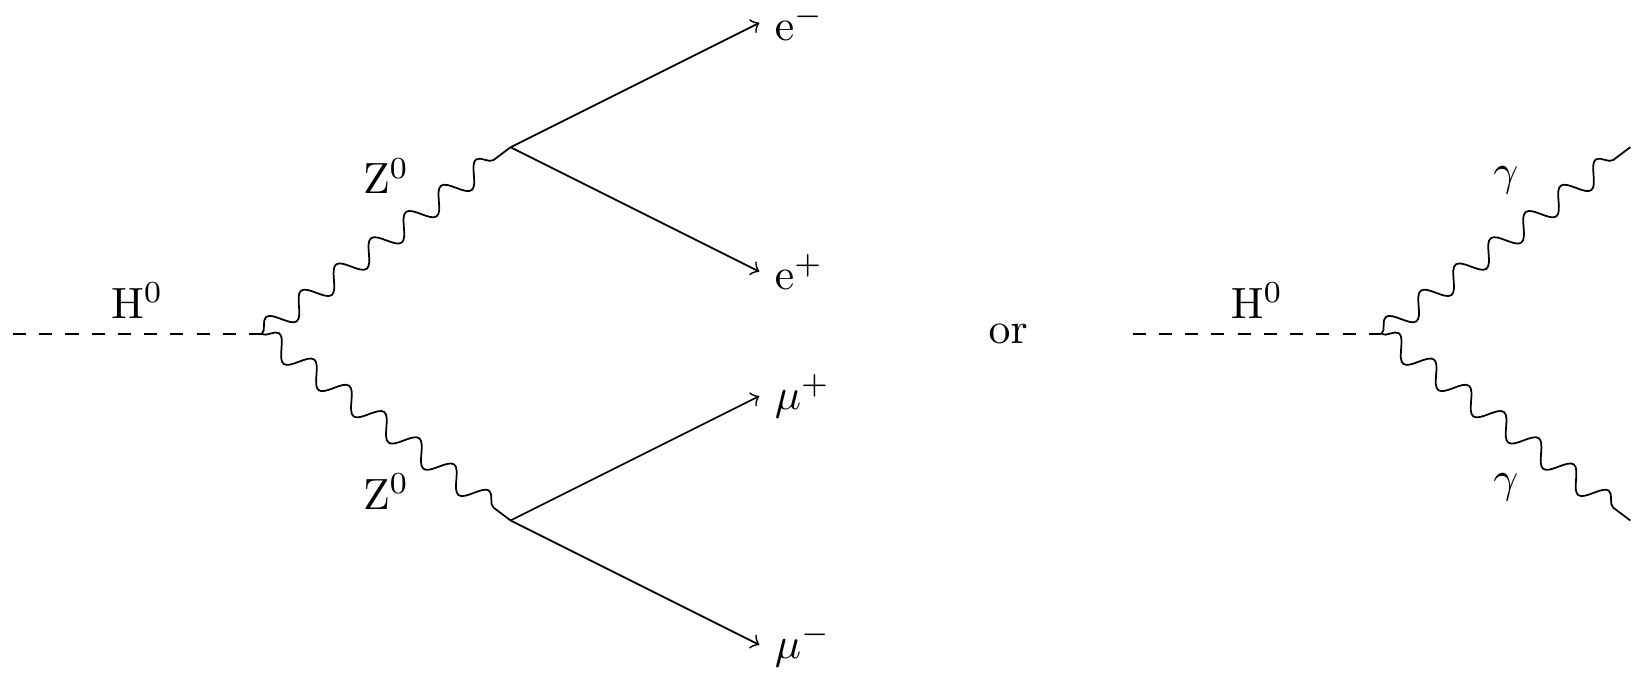
\includegraphics[scale=0.2]{HiggsDecay}
\end{center}

\subsection*{Feynman Diagrams}

\begin{center}
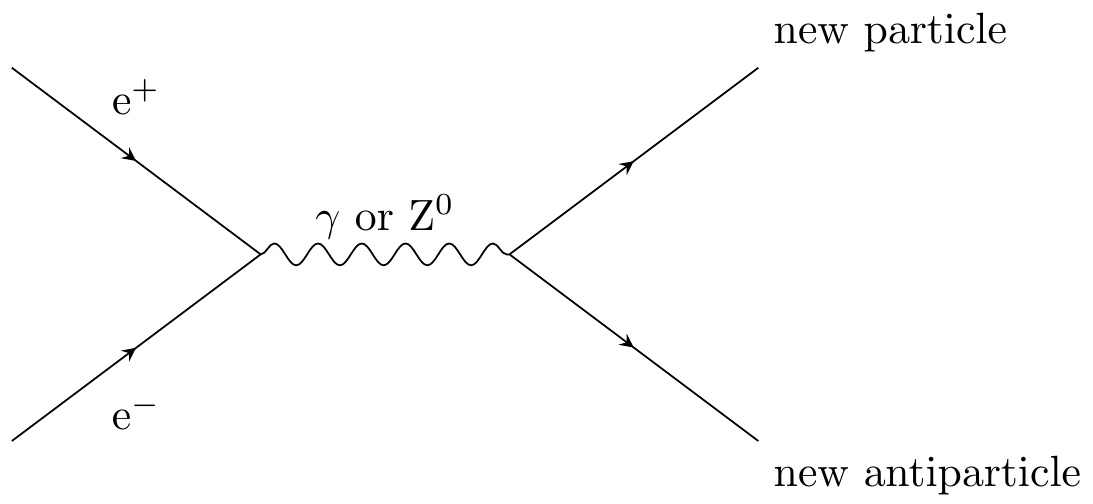
\includegraphics[scale=0.25]{Anihilation}
\end{center}

Electrons and positrons aren't quarks so this can't occur by the strong force. The total charge going in is 0 so the exchange particle must be neutral. This means that it is either a photon or a \zboson. Since it is a virtual particle it must eventually decay.

When drawing a Feynman diagram the typical axis are time increases upwards and space increases to the right. This means that if you rotate a diagram \SI{90}{\degree} clockwise and make all arrows going backwards into antiparticles then you get two equivalent diagrams

\begin{center}
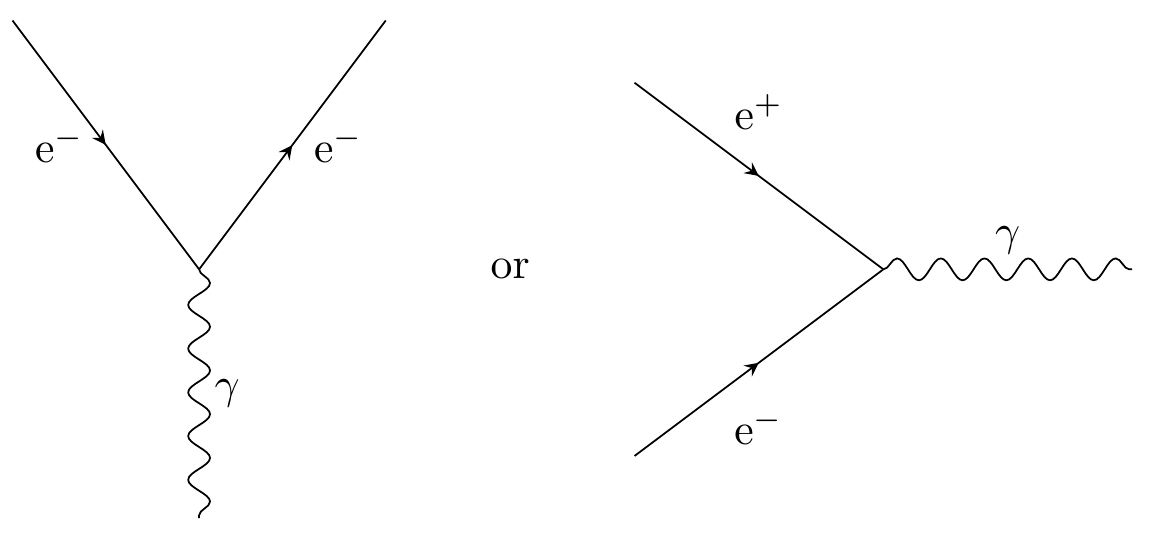
\includegraphics[scale=0.25]{AnihilationOrRedirect}
\end{center}

In Feynman diagrams it is standard to have antiparticles with their arrows going backwards in time.

\subsection*{Conservation Laws}

Some quantities are conserved in all (or at least most) reactions. This includes
\begin{itemize}
\item Charge (\(Q\) or \(C\))
\item Lepton number (\(L\)). Also each individual lepton generation number
\begin{itemize}
\item Electron number (\(L_\mathrm{e}\))
\item Muon number (\(L_\mu\))
\item Tauon number (\(L_\tau\))
\end{itemize}
\item Baryon number (\(B\))
\item Energy (\(E\))
\item Momentum (\(p\))
\end{itemize}

\begin{center}
\begin{tabular}{c|ccc}\hline
Number & +1 & 0 & -1\\\hline
\(L\) & \electron, \muonm, \tauonm & All other particles & \positron, \muonp, \tauonp\\
 & \neutrino[e], \neutrino[\mu], \neutrino[\tau] & & \antineutrino[e], \antineutrino[\mu], \antineutrino[\tau]\\\hline
\(L_e\) & \electron, \neutrino[e] & All other particles & \positron, \antineutrino[e]\\\hline
\(L_\mu\) & \muonm, \neutrino[\mu] & All other particles & \muonp, \antineutrino[\mu]\\\hline
\(L_\tau\) & \tauonm, \neutrino[\tau] & All other particles & \tauonp, \antineutrino[\tau]\\\hline
\(B\) & Baryons (3 quarks) & All other particles & Antibaryons (3 antiquarks)\\\hline
\end{tabular}
\end{center}
From this we give quarks a baryon number of \(+\frac 13\) and antiquarks a baryon number of \(-\frac 13\). This means that mesons (\quark\antiquark) have a baryon number of \(\frac 13-\frac 13=0\). Meson number is not a conserved number.

\section{}

Only the weak force can change quark flavour.

\begin{center}
\begin{tabular}{ccc}\hline
Force & Acts on & Relative Strength\\\hline
Strong force & Quarks and gluons & 1\\
EM & Charged particles & \num{e-2}\\
Weak & Fermions & \num{e-10	}\\
Gravity & Particles with mass & \num{e-40}\\\hline
\end{tabular}
\end{center}

Above a certain energy EM and weak forces are equally strong as there is so much energy that making a a photon or a \wpm/\zboson is just as easy so EM and weak forces merge into the electroweak (EW) force. We also think that the same happens with the strong force at even higher temperatures.

\begin{center}
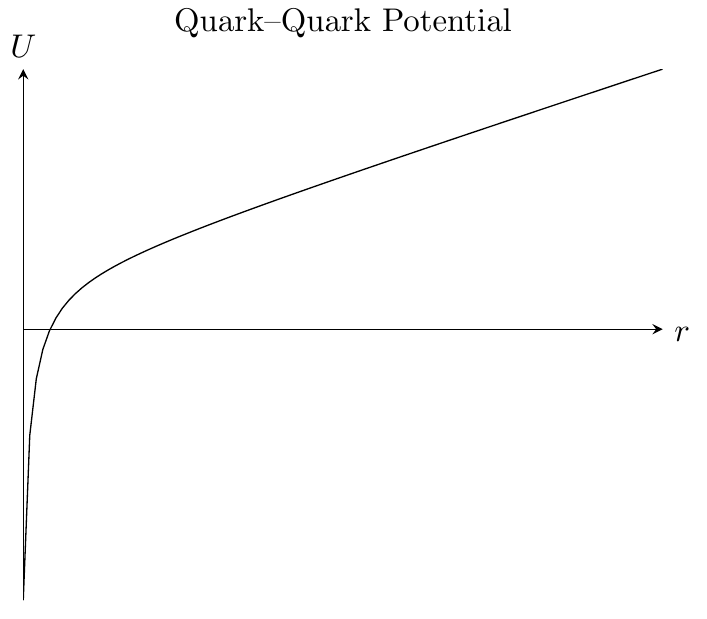
\includegraphics[scale=0.3]{QuarkQuarkPotential}
\end{center}

The quark--quark potential doesn't depend significantly on flavour, colour or whether it is a particle or antiparticle. Separating two quarks requires a lot of energy. This energy will form new particles which will then separate into multiple multi-quark systems rather than a single quark. This is called quark confinement.
\[\up\bar\up\ce{->}\up\quad\bar\up\ce{->}\up\bar\up\qquad\qquad\up\bar\up\]

\subsection*{Astrophysics}

\subsubsection*{Red/Blue Shift}

\[\frac{\lambda_{\mathrm{observed}}}{\lambda_{\mathrm{source}}}=\sqrt{\frac{1+v/c}{1-v/c}}\]
Where \(v\) is the relative speed between the observer and the source and \(v>0\) if they are moving appart. For \(v\ll c\) this reduces to
\[\frac{\Delta\lambda}{\lambda_{\mathrm{source}}}\approx\frac vc\]
Redshift \(z\) is a numerical value
\[z=\frac{\lambda_{\mathrm{obsv}}-\lambda_{\mathrm{source}}}{\lambda_{\mathrm{source}}}=\frac{f_{\mathrm{source}}-f_{\mathrm{obsv}}}{f_{\mathrm{obsv}}}\]
\[1+z=\frac{\lambda_{\mathrm{obsv}}}{\lambda_{\mathrm{source}}}=\frac{f_{\mathrm{source}}}{f_{\mathrm{obsv}}}\]

1 parsec (pc) \(\approx\) 3.3 light years (ly) \(\approx\num{3.086e16}\,\si{m}\)

Measurement of redshift of distant stars/galaxies shows that their velocity \(v\) is roughly proportional to the distance from us
\[v\propto r\implies v=H_0 r\]
where \(H_0\) is hubbles constant, \(H_0=\num{2.3e-18}\,\si{s^{-1}}\approx\SI{70}{kms^{-1}/Mpc}\). With all but a few local exceptions these galaxies are moving away from us.
\begin{example}
How far away is a galaxy with redshift \(z=0.1?\)

\[v=\num{3e7}\implies r=\frac{v}{H_0}=\num{1.3e25}\,\si{m}=\num{1.4e9}\,\si{ly}\]
\end{example}

Not only are all galaxies moving away from us but they are moving away from every thing else. The universe is growing isotropically (equally in all directions). This means the universe is expanding. This tracks back to the universe having 0 size at some point. Projecting backwards \(H_0^{-1}\approx14\) billion years which is a very basic approximation of the age of the universe. There is no center of the universe meaning the big bang happened everywhere simultaneously.

Gravity will slow expansion so the amount of gravity (and therefore matter) will affect the future of the universe. Is there enough matter to stop the universe from collapsing is an important question.

\section{}

A more sophisticated prediction for the future of the universe depends on how much gravity there is. This depends on how the universe compares to a critical density \(\rho_c\). A classical calculation gives
\[\rho_c=\frac{3H_0^2}{8\pi G}\]
The ratio of the actual density of the universe to this critical density is
\[\Omega=\frac{\rho}{\rho_c}\]
If the universe collapses it is called closed and \(\rho>\rho_c\implies\Omega>1\)

If the universe expands forever it is called open and \(\rho<\rho_c\implies\Omega<1\)

If the universe expands but stops after an infinite amount of time it is called flat and \(\rho=\rho_c\implies\Omega=1\)

\begin{center}
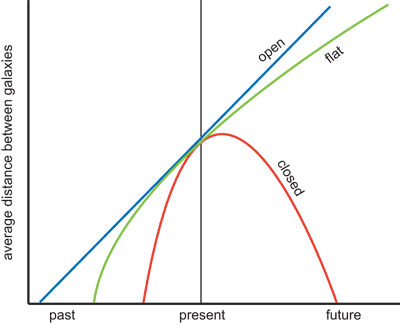
\includegraphics[scale=0.6]{FateOfTheUniverse}
\end{center}

If the universe is empty then the time from the start of the universe is \(H_0^{-1}\) seconds. If it is flat then it is \(\frac 23 H_0^{-1}\) seconds. One piece of evidence that the universe is flat is that the sum of all angles of a triangle in space time is \SI{180}{\degree}. A lot of evidence agrees that the universe is flat.

Our best guess for the age of the universe is \(13.799\pm0.021\) billion years old.

At the big bang the universe was very hot and very dense. At Planck scales quantum mechanics and general relativity break down. 

Before \num{e-37} \si{s} it is unknown what happened. Before \num{e-11} \si{s} it is uncertain what happened.

\(\sim\num{e-37}\) to \(\sim\num{e-32}\) the universe was undergoing inflation. The universe expanded very rapidly, by a factor of \num{e78}. This means that its speed was much greater than the speed of light. This is allowed as no matter went at this speed just the universe. This means that things became causally disconnected.

At \num{e-32} \si{s} inflation stops and the pressure/momentum causes expansion. The universe cools because it is expanding. At this point only quarks, gluons and photons can form.

At \num{e-12} \si{s} weak and EM split as the energy \(E \approx \SI{e-8}{\joule} \approx \SI{90}{GeV} \approx m_{\wpm,\zboson}c^2\).

At \num{e-6} \si{s} it is cool enough to form neutrons and protons as the energy \(E\approx\SI{1}{GeV}\approx m_{p,n}c^2\) \((T\approx\num{e13}\,\si{K})\).

At 3 min it is cool enough to form elements (without electrons) as the energy \(E \approx \SI{1}{MeV} \approx BE(\ce{H})\) \((T\approx\num{e10}\,\si{K})\).

At 10 min it's too cool to overcome the Coulomb barrier so new elements can't form. The universe is 75\% \ce{H}, 25\% \ce{He} and trace other elements.

At \num{380000} years it is cool enough that atoms (with electrons) because the energy \(E < IE\) \((T\approx\SI{3000}{K})\).

In the big bang hydrogen and helium were made. We can work out the total amount of baryonic matter \(\rho_{\mathrm{bar}}/\rho_c = \Omega_{\mathrm{bar}} = 0.04\) since baryon number is conserved this is the same today.

After about 1 billion years hydrogen and helium come together under their own gravity. This contraction causes them to heat up.

One unit commonly used in astrophysics is a solar mass which is the mass of the sun and is equivalent to \num{2e30} \si{kg} and has the symbol \si{\solarmass}.

For sustained \ce{H} fusion we need \(M>\SI{0.08}{\solarmass}\). Once the star runs out of \ce{H} fusion stops so radiation pressure is lost so the star shrinks so it gets hotter. If \(M>\SI{0.5}{\solarmass}\) then \ce{He} fusion can occur and the star gets larger so the outer layers cool. This is a red giant. If it is heavy enough fusion of heavier elements occurs up to \ce{^56Fe}/\ce{^56Ni}. To get all the way to iron we need \(M>\SI{8}{\solarmass}\).

In supernovae and neutron star merges elements with atomic mass greater tha 56 can be formed.

\begin{center}
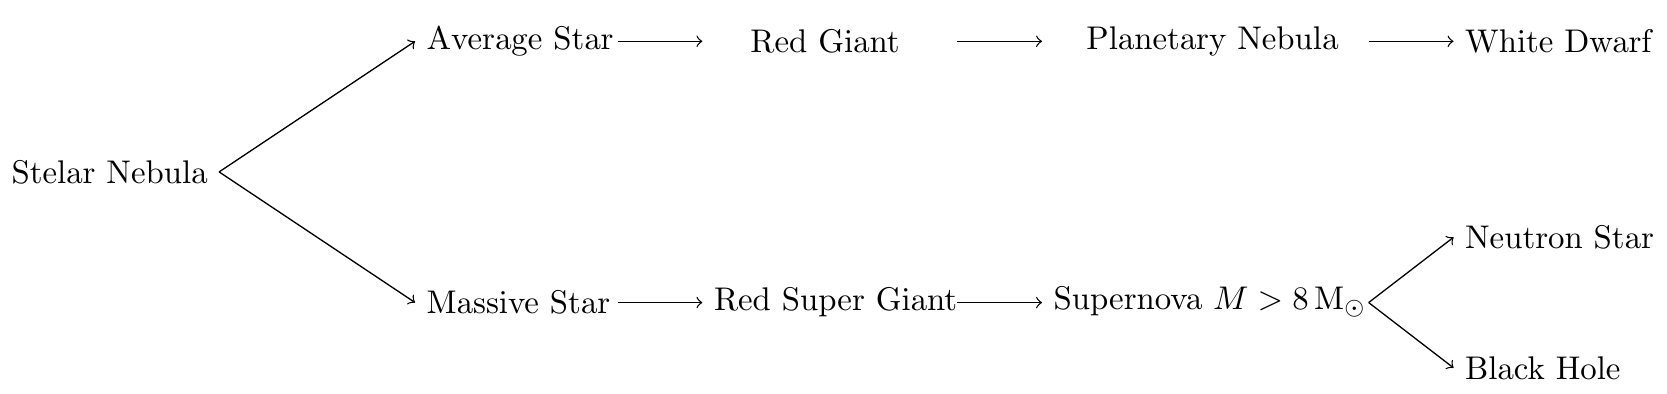
\includegraphics[scale=0.3]{LifeOfAStar}
\end{center}

\section{}

\begin{center}
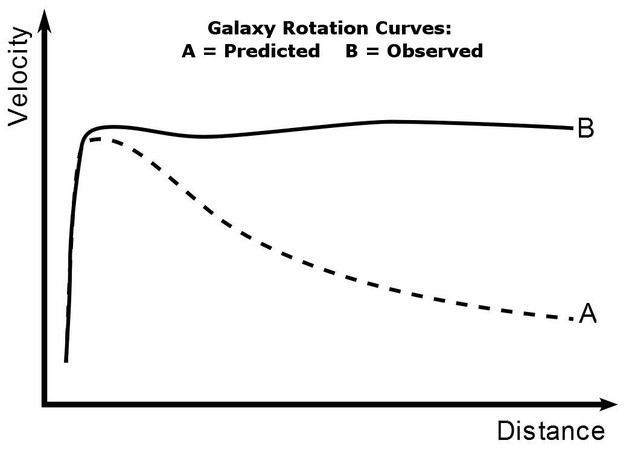
\includegraphics[scale=0.4]{GalaxyRotationSpeed}
\end{center}

For a spinning galaxy at a small distance \(r\) from the centre we expect that the velocity, \(v\), is proportional to \(r\), \(v\propto r\). For a large distance we expect that equating centripetal and gravitational forces give the speed
\[\frac{mv^2}{r}=\frac{Gm_1m_2}{r^2}\implies v\propto\frac{1}{\sqrt{r}}\]
Our observation of the speed of the galaxy at these distances is higher than expected. This means that there must be more force than just the gravity of the rest of the galaxy which means that there must be more matter which we can't see so we call it dark matter. Dark matter is probably in a halo around the galaxy. The density ratio of visible matter is \(\Omega_\mathrm{lum}=0.03\). The density ratio of dark matter is \(\Omega_\mathrm{DM}=0.23\) which is about 8 times as much as visible matter.

No particle in the standard model fits the prediction of dark matter which is that it doesn't interact by the strong or EM force and hardly by the weak force if at all but is also very stable and much heavier than a neutrino. (It is possible that if we have measured the mass of a neutrino incorrectly or made an error in predicting the number of neutrinos that dark matter is neutrinos).

Super symmetry (SUSY) is a best guess at an extension for the standard model. It predicts every particle has a super symmetric counter part known as an sparticle (e.g., a super symmetric quark is a squark, a supper symmetric lepton is a slepton) these have a different spin by \(\frac 12\) and solve some problems with the standard model.

To try to detect dark matter we put very sensitive detectors deep underground (to eliminate back ground radiation) we predict dark matter will interact a tiny bit by the weak force and if it does we should eventually detect it.

Some possible explanations for dark matter are
\begin{itemize}
\item WIMPS - weakly interacting massive particles
\item Pre-inflation black holes
\item Axions - particles needed to explain the lack of CP violation in most strong interactions
\item Modified gravity - general relativity doesn't work (unlikely)
\item Negative mass matter - mathematically allowed (probably, it could also be a bug in the code that did the computation)
\item Super symmetry
\end{itemize}

\subsection*{Binary Stellar Systems}

Binary stellar systems are what cause type 1a supernovae. A binary system is two stars orbiting each other. Typically they have masses in the range \(\SI{1}{\solarmass}<M<\SI{8}{\solarmass}\) and one of them is much heavier than the other so it evolves faster. After the hydrogen runs out the helium burns and it becomes a red giant. The smaller star becomes a white dwarf. Some layers from the red giant transfer to the white dwarf. When the mass of the white dwarf reaches \SI{1.44}{\solarmass} (Chandrasekhar limit) it implodes under its own weight as a type 1a supernova.

Since this occurs due to fundamental nuclear physics the explosions are almost identical for any 2 type 1a supernovae. This means that using their observed brightness we can tell how far away they are. We call a type 1a supernova a standard candle.

In 1998 scientists were studying distant (\(z=1\)) type 1a supernovae. The distance can be measured based on brightness and the speed can be calculated based on their redshift. The galaxies were receding more faster than hubbles law predicts. This suggests distant things are accelerating away from us. To explain this we introduce dark energy. The density ratio of dark energy is \(\Omega_\lambda=0.73\). This means that the total ratio of densities is
\[\Omega_\mathrm{tot}=\Omega_\mathrm{bar}+\Omega_\mathrm{DM}+\Omega_\lambda=0.04+0.23+0.73=1.00\]
This means that the energy of the universe is 73\% dark energy, 23\% dark matter and 4\% normal matter which includes about 0.5\% stars and 0.3\% neutrinos. The fact that dark energy causes acceleration means that even if \(\Omega_\mathrm{tot}=1\) the universe will still be open and expand forever.

It is possible that dark matter and dark energy are the same. Dark matter explains galactic scale motion and dark energy explains universe scale motion. Dark energy is a lot like inflation.

There are several goals in physics of finding a combined theory of the different forces.
\begin{itemize}
\item EM + weak force = Electroweak theory (EW) [well understood, explains things like how the Higgs boson works to give mass]
\item EW + strong force = Grand unified theory (GUT) [various models, not agreed upon]
\item GUT + gravity = Theory of everything (TOE) [string theory? supersymmetry? probably not :(\kern0.1em]
\end{itemize}
%\end{document}